\documentclass[1p]{elsarticle_modified}
%\bibliographystyle{elsarticle-num}

%\usepackage[colorlinks]{hyperref}
%\usepackage{abbrmath_seonhwa} %\Abb, \Ascr, \Acal ,\Abf, \Afrak
\usepackage{amsfonts}
\usepackage{amssymb}
\usepackage{amsmath}
\usepackage{amsthm}
\usepackage{scalefnt}
\usepackage{amsbsy}
\usepackage{kotex}
\usepackage{caption}
\usepackage{subfig}
\usepackage{color}
\usepackage{graphicx}
\usepackage{xcolor} %% white, black, red, green, blue, cyan, magenta, yellow
\usepackage{float}
\usepackage{setspace}
\usepackage{hyperref}

\usepackage{tikz}
\usetikzlibrary{arrows}

\usepackage{multirow}
\usepackage{array} % fixed length table
\usepackage{hhline}

%%%%%%%%%%%%%%%%%%%%%
\makeatletter
\renewcommand*\env@matrix[1][\arraystretch]{%
	\edef\arraystretch{#1}%
	\hskip -\arraycolsep
	\let\@ifnextchar\new@ifnextchar
	\array{*\c@MaxMatrixCols c}}
\makeatother %https://tex.stackexchange.com/questions/14071/how-can-i-increase-the-line-spacing-in-a-matrix
%%%%%%%%%%%%%%%

\usepackage[normalem]{ulem}

\newcommand{\msout}[1]{\ifmmode\text{\sout{\ensuremath{#1}}}\else\sout{#1}\fi}
%SOURCE: \msout is \stkout macro in https://tex.stackexchange.com/questions/20609/strikeout-in-math-mode

\newcommand{\cancel}[1]{
	\ifmmode
	{\color{red}\msout{#1}}
	\else
	{\color{red}\sout{#1}}
	\fi
}

\newcommand{\add}[1]{
	{\color{blue}\uwave{#1}}
}

\newcommand{\replace}[2]{
	\ifmmode
	{\color{red}\msout{#1}}{\color{blue}\uwave{#2}}
	\else
	{\color{red}\sout{#1}}{\color{blue}\uwave{#2}}
	\fi
}

\newcommand{\Sol}{\mathcal{S}} %segment
\newcommand{\D}{D} %diagram
\newcommand{\A}{\mathcal{A}} %arc


%%%%%%%%%%%%%%%%%%%%%%%%%%%%%5 test

\def\sl{\operatorname{\textup{SL}}(2,\Cbb)}
\def\psl{\operatorname{\textup{PSL}}(2,\Cbb)}
\def\quan{\mkern 1mu \triangleright \mkern 1mu}

\theoremstyle{definition}
\newtheorem{thm}{Theorem}[section]
\newtheorem{prop}[thm]{Proposition}
\newtheorem{lem}[thm]{Lemma}
\newtheorem{ques}[thm]{Question}
\newtheorem{cor}[thm]{Corollary}
\newtheorem{defn}[thm]{Definition}
\newtheorem{exam}[thm]{Example}
\newtheorem{rmk}[thm]{Remark}
\newtheorem{alg}[thm]{Algorithm}

\newcommand{\I}{\sqrt{-1}}
\begin{document}

%\begin{frontmatter}
%
%\title{Boundary parabolic representations of knots up to 8 crossings}
%
%%% Group authors per affiliation:
%\author{Yunhi Cho} 
%\address{Department of Mathematics, University of Seoul, Seoul, Korea}
%\ead{yhcho@uos.ac.kr}
%
%
%\author{Seonhwa Kim} %\fnref{s_kim}}
%\address{Center for Geometry and Physics, Institute for Basic Science, Pohang, 37673, Korea}
%\ead{ryeona17@ibs.re.kr}
%
%\author{Hyuk Kim}
%\address{Department of Mathematical Sciences, Seoul National University, Seoul 08826, Korea}
%\ead{hyukkim@snu.ac.kr}
%
%\author{Seokbeom Yoon}
%\address{Department of Mathematical Sciences, Seoul National University, Seoul, 08826,  Korea}
%\ead{sbyoon15@snu.ac.kr}
%
%\begin{abstract}
%We find all boundary parabolic representation of knots up to 8 crossings.
%
%\end{abstract}
%\begin{keyword}
%    \MSC[2010] 57M25 
%\end{keyword}
%
%\end{frontmatter}

%\linenumbers
%\tableofcontents
%
\newcommand\colored[1]{\textcolor{white}{\rule[-0.35ex]{0.8em}{1.4ex}}\kern-0.8em\color{red} #1}%
%\newcommand\colored[1]{\textcolor{white}{ #1}\kern-2.17ex	\textcolor{white}{ #1}\kern-1.81ex	\textcolor{white}{ #1}\kern-2.15ex\color{red}#1	}

{\Large $\underline{12a_{0012}~(K12a_{0012})}$}

\setlength{\tabcolsep}{10pt}
\renewcommand{\arraystretch}{1.6}
\vspace{1cm}\begin{tabular}{m{100pt}>{\centering\arraybackslash}m{274pt}}
\multirow{5}{120pt}{
	\centering
	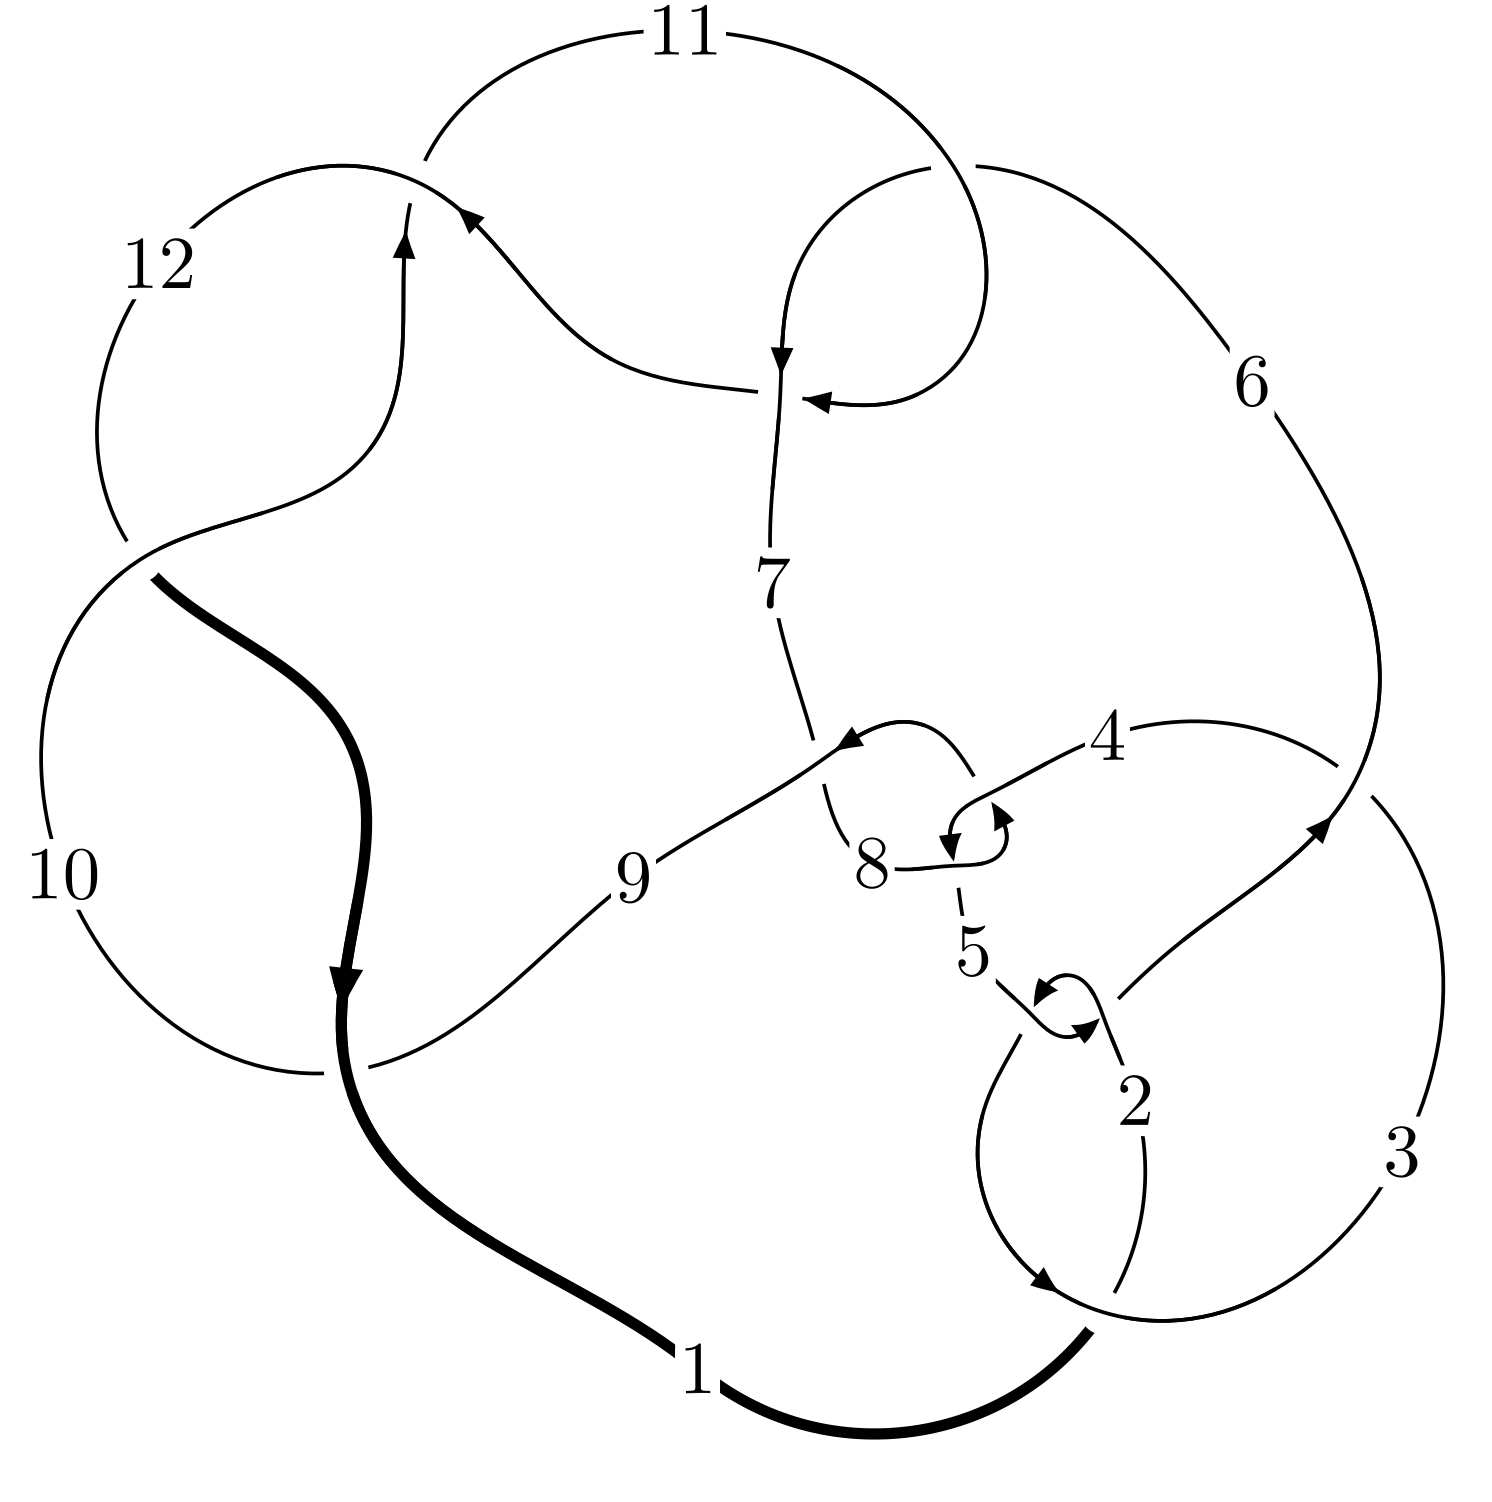
\includegraphics[width=112pt]{../../../GIT/diagram.site/Diagrams/png/813_12a_0012.png}\\
\ \ \ A knot diagram\footnotemark}&
\allowdisplaybreaks
\textbf{Linearized knot diagam} \\
\cline{2-2}
 &
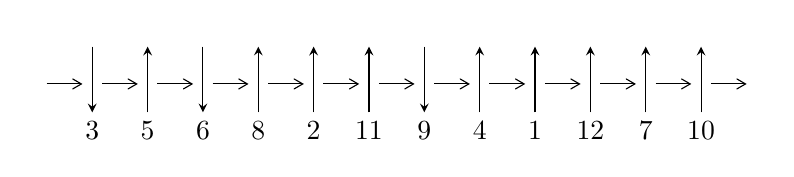
\begin{tikzpicture}[x=20pt, y=17pt]
	% nodes
	\node (C0) at (0, 0) {};
	\node (C1) at (1, 0) {};
	\node (C1U) at (1, +1) {};
	\node (C1D) at (1, -1) {3};

	\node (C2) at (2, 0) {};
	\node (C2U) at (2, +1) {};
	\node (C2D) at (2, -1) {5};

	\node (C3) at (3, 0) {};
	\node (C3U) at (3, +1) {};
	\node (C3D) at (3, -1) {6};

	\node (C4) at (4, 0) {};
	\node (C4U) at (4, +1) {};
	\node (C4D) at (4, -1) {8};

	\node (C5) at (5, 0) {};
	\node (C5U) at (5, +1) {};
	\node (C5D) at (5, -1) {2};

	\node (C6) at (6, 0) {};
	\node (C6U) at (6, +1) {};
	\node (C6D) at (6, -1) {11};

	\node (C7) at (7, 0) {};
	\node (C7U) at (7, +1) {};
	\node (C7D) at (7, -1) {9};

	\node (C8) at (8, 0) {};
	\node (C8U) at (8, +1) {};
	\node (C8D) at (8, -1) {4};

	\node (C9) at (9, 0) {};
	\node (C9U) at (9, +1) {};
	\node (C9D) at (9, -1) {1};

	\node (C10) at (10, 0) {};
	\node (C10U) at (10, +1) {};
	\node (C10D) at (10, -1) {12};

	\node (C11) at (11, 0) {};
	\node (C11U) at (11, +1) {};
	\node (C11D) at (11, -1) {7};

	\node (C12) at (12, 0) {};
	\node (C12U) at (12, +1) {};
	\node (C12D) at (12, -1) {10};
	\node (C13) at (13, 0) {};

	% arrows
	\draw[->,>={angle 60}]
	(C0) edge (C1) (C1) edge (C2) (C2) edge (C3) (C3) edge (C4) (C4) edge (C5) (C5) edge (C6) (C6) edge (C7) (C7) edge (C8) (C8) edge (C9) (C9) edge (C10) (C10) edge (C11) (C11) edge (C12) (C12) edge (C13) ;	\draw[->,>=stealth]
	(C1U) edge (C1D) (C2D) edge (C2U) (C3U) edge (C3D) (C4D) edge (C4U) (C5D) edge (C5U) (C6D) edge (C6U) (C7U) edge (C7D) (C8D) edge (C8U) (C9D) edge (C9U) (C10D) edge (C10U) (C11D) edge (C11U) (C12D) edge (C12U) ;
	\end{tikzpicture} \\
\hhline{~~} \\& 
\textbf{Solving Sequence} \\ \cline{2-2} 
 &
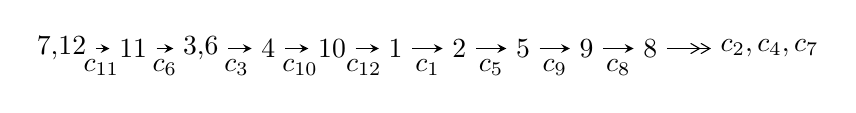
\begin{tikzpicture}[x=23pt, y=7pt]
	% node
	\node (A0) at (-1/8, 0) {7,12};
	\node (A1) at (1, 0) {11};
	\node (A2) at (33/16, 0) {3,6};
	\node (A3) at (25/8, 0) {4};
	\node (A4) at (33/8, 0) {10};
	\node (A5) at (41/8, 0) {1};
	\node (A6) at (49/8, 0) {2};
	\node (A7) at (57/8, 0) {5};
	\node (A8) at (65/8, 0) {9};
	\node (A9) at (73/8, 0) {8};
	\node (C1) at (1/2, -1) {$c_{11}$};
	\node (C2) at (3/2, -1) {$c_{6}$};
	\node (C3) at (21/8, -1) {$c_{3}$};
	\node (C4) at (29/8, -1) {$c_{10}$};
	\node (C5) at (37/8, -1) {$c_{12}$};
	\node (C6) at (45/8, -1) {$c_{1}$};
	\node (C7) at (53/8, -1) {$c_{5}$};
	\node (C8) at (61/8, -1) {$c_{9}$};
	\node (C9) at (69/8, -1) {$c_{8}$};
	\node (A10) at (11, 0) {$c_{2},c_{4},c_{7}$};

	% edge
	\draw[->,>=stealth]	
	(A0) edge (A1) (A1) edge (A2) (A2) edge (A3) (A3) edge (A4) (A4) edge (A5) (A5) edge (A6) (A6) edge (A7) (A7) edge (A8) (A8) edge (A9) ;
	\draw[->>,>={angle 60}]	
	(A9) edge (A10);
\end{tikzpicture} \\ 

\end{tabular} \\

\footnotetext{
The image of knot diagram is generated by the software ``\textbf{Draw programme}" developed by Andrew Bartholomew(\url{http://www.layer8.co.uk/maths/draw/index.htm\#Running-draw}), where we modified some parts for our purpose(\url{https://github.com/CATsTAILs/LinksPainter}).
}\phantom \\ \newline 
\centering \textbf{Ideals for irreducible components\footnotemark of $X_{\text{par}}$} 
 
\begin{align*}
I^u_{1}&=\langle 
3 u^{88}-2 u^{87}+\cdots+2 b-4,\;-3 u^{88}+6 u^{87}+\cdots+2 a-5,\;u^{89}-3 u^{88}+\cdots+3 u^2-1\rangle \\
I^u_{2}&=\langle 
- u^2 a- a u+b,\;a^2- a u+u^2,\;u^3+u^2-1\rangle \\
\\
\end{align*}
\raggedright * 2 irreducible components of $\dim_{\mathbb{C}}=0$, with total 95 representations.\\
\footnotetext{All coefficients of polynomials are rational numbers. But the coefficients are sometimes approximated in decimal forms when there is not enough margin.}
\newpage
\renewcommand{\arraystretch}{1}
\centering \section*{I. $I^u_{1}= \langle 3 u^{88}-2 u^{87}+\cdots+2 b-4,\;-3 u^{88}+6 u^{87}+\cdots+2 a-5,\;u^{89}-3 u^{88}+\cdots+3 u^2-1 \rangle$}
\flushleft \textbf{(i) Arc colorings}\\
\begin{tabular}{m{7pt} m{180pt} m{7pt} m{180pt} }
\flushright $a_{7}=$&$\begin{pmatrix}0\\u\end{pmatrix}$ \\
\flushright $a_{12}=$&$\begin{pmatrix}1\\0\end{pmatrix}$ \\
\flushright $a_{11}=$&$\begin{pmatrix}1\\u^2\end{pmatrix}$ \\
\flushright $a_{3}=$&$\begin{pmatrix}\frac{3}{2} u^{88}-3 u^{87}+\cdots-\frac{11}{2} u^2+\frac{5}{2}\\-\frac{3}{2} u^{88}+u^{87}+\cdots+u+2\end{pmatrix}$ \\
\flushright $a_{6}=$&$\begin{pmatrix}- u\\- u^3+u\end{pmatrix}$ \\
\flushright $a_{4}=$&$\begin{pmatrix}4 u^{88}-8 u^{87}+\cdots-10 u^2+3\\-3 u^{88}+\frac{1}{2} u^{87}+\cdots+\frac{7}{2} u+4\end{pmatrix}$ \\
\flushright $a_{10}=$&$\begin{pmatrix}- u^2+1\\u^2\end{pmatrix}$ \\
\flushright $a_{1}=$&$\begin{pmatrix}u^4- u^2+1\\- u^4\end{pmatrix}$ \\
\flushright $a_{2}=$&$\begin{pmatrix}\frac{1}{2} u^{88}- u^{87}+\cdots- u+\frac{1}{2}\\-\frac{1}{2} u^{88}+u^{87}+\cdots+\frac{1}{2} u^2+u\end{pmatrix}$ \\
\flushright $a_{5}=$&$\begin{pmatrix}4 u^{88}-8 u^{87}+\cdots- u+1\\-2 u^{88}+\frac{1}{2} u^{87}+\cdots+u^2+\frac{9}{2} u\end{pmatrix}$ \\
\flushright $a_{9}=$&$\begin{pmatrix}- u^6+u^4-2 u^2+1\\u^6+u^2\end{pmatrix}$ \\
\flushright $a_{8}=$&$\begin{pmatrix}- u^{13}+2 u^{11}-5 u^9+6 u^7-6 u^5+4 u^3- u\\u^{13}- u^{11}+3 u^9-2 u^7+2 u^5- u^3+u\end{pmatrix}$\\&\end{tabular}
\flushleft \textbf{(ii) Obstruction class $= -1$}\\~\\
\flushleft \textbf{(iii) Cusp Shapes $= \frac{9}{2} u^{88}-7 u^{87}+\cdots+10 u+\frac{25}{2}$}\\~\\
\newpage\renewcommand{\arraystretch}{1}
\flushleft \textbf{(iv) u-Polynomials at the component}\newline \\
\begin{tabular}{m{50pt}|m{274pt}}
Crossings & \hspace{64pt}u-Polynomials at each crossing \\
\hline $$\begin{aligned}c_{1}\end{aligned}$$&$\begin{aligned}
&u^{89}+42 u^{88}+\cdots+31 u-1
\end{aligned}$\\
\hline $$\begin{aligned}c_{2},c_{5}\end{aligned}$$&$\begin{aligned}
&u^{89}+4 u^{88}+\cdots- u-1
\end{aligned}$\\
\hline $$\begin{aligned}c_{3}\end{aligned}$$&$\begin{aligned}
&u^{89}-4 u^{88}+\cdots+14621 u-1153
\end{aligned}$\\
\hline $$\begin{aligned}c_{4},c_{8}\end{aligned}$$&$\begin{aligned}
&u^{89}- u^{88}+\cdots+224 u-64
\end{aligned}$\\
\hline $$\begin{aligned}c_{6},c_{11}\end{aligned}$$&$\begin{aligned}
&u^{89}-3 u^{88}+\cdots+3 u^2-1
\end{aligned}$\\
\hline $$\begin{aligned}c_{7}\end{aligned}$$&$\begin{aligned}
&u^{89}+35 u^{88}+\cdots-68608 u-4096
\end{aligned}$\\
\hline $$\begin{aligned}c_{9},c_{10},c_{12}\end{aligned}$$&$\begin{aligned}
&u^{89}-23 u^{88}+\cdots+6 u-1
\end{aligned}$\\
\hline
\end{tabular}\\~\\
\newpage\renewcommand{\arraystretch}{1}
\flushleft \textbf{(v) Riley Polynomials at the component}\newline \\
\begin{tabular}{m{50pt}|m{274pt}}
Crossings & \hspace{64pt}Riley Polynomials at each crossing \\
\hline $$\begin{aligned}c_{1}\end{aligned}$$&$\begin{aligned}
&y^{89}+14 y^{88}+\cdots+1271 y-1
\end{aligned}$\\
\hline $$\begin{aligned}c_{2},c_{5}\end{aligned}$$&$\begin{aligned}
&y^{89}+42 y^{88}+\cdots+31 y-1
\end{aligned}$\\
\hline $$\begin{aligned}c_{3}\end{aligned}$$&$\begin{aligned}
&y^{89}-14 y^{88}+\cdots+87088919 y-1329409
\end{aligned}$\\
\hline $$\begin{aligned}c_{4},c_{8}\end{aligned}$$&$\begin{aligned}
&y^{89}+35 y^{88}+\cdots-68608 y-4096
\end{aligned}$\\
\hline $$\begin{aligned}c_{6},c_{11}\end{aligned}$$&$\begin{aligned}
&y^{89}-23 y^{88}+\cdots+6 y-1
\end{aligned}$\\
\hline $$\begin{aligned}c_{7}\end{aligned}$$&$\begin{aligned}
&y^{89}+27 y^{88}+\cdots+739246080 y-16777216
\end{aligned}$\\
\hline $$\begin{aligned}c_{9},c_{10},c_{12}\end{aligned}$$&$\begin{aligned}
&y^{89}+89 y^{88}+\cdots+46 y-1
\end{aligned}$\\
\hline
\end{tabular}\\~\\
\newpage\flushleft \textbf{(vi) Complex Volumes and Cusp Shapes}
$$\begin{array}{c|c|c}  
\text{Solutions to }I^u_{1}& \I (\text{vol} + \sqrt{-1}CS) & \text{Cusp shape}\\
 \hline 
\begin{aligned}
u &= \phantom{-}0.984195 + 0.195609 I \\
a &= \phantom{-}0.284066 + 0.070833 I \\
b &= -0.868179 - 0.697870 I\end{aligned}
 & \phantom{-}3.78188 - 0.84858 I & \phantom{-0.000000 } 0 \\ \hline\begin{aligned}
u &= \phantom{-}0.984195 - 0.195609 I \\
a &= \phantom{-}0.284066 - 0.070833 I \\
b &= -0.868179 + 0.697870 I\end{aligned}
 & \phantom{-}3.78188 + 0.84858 I & \phantom{-0.000000 } 0 \\ \hline\begin{aligned}
u &= \phantom{-}0.939086 + 0.312963 I \\
a &= -1.39245 - 1.37113 I \\
b &= \phantom{-}0.291029 + 0.718996 I\end{aligned}
 & \phantom{-}2.25621 + 6.04954 I & \phantom{-0.000000 } 0 \\ \hline\begin{aligned}
u &= \phantom{-}0.939086 - 0.312963 I \\
a &= -1.39245 + 1.37113 I \\
b &= \phantom{-}0.291029 - 0.718996 I\end{aligned}
 & \phantom{-}2.25621 - 6.04954 I & \phantom{-0.000000 } 0 \\ \hline\begin{aligned}
u &= -0.946105 + 0.284359 I \\
a &= \phantom{-}0.0319019 - 0.1300720 I \\
b &= -0.790886 + 1.103430 I\end{aligned}
 & \phantom{-}3.90708 - 4.17956 I & \phantom{-0.000000 } 0 \\ \hline\begin{aligned}
u &= -0.946105 - 0.284359 I \\
a &= \phantom{-}0.0319019 + 0.1300720 I \\
b &= -0.790886 - 1.103430 I\end{aligned}
 & \phantom{-}3.90708 + 4.17956 I & \phantom{-0.000000 } 0 \\ \hline\begin{aligned}
u &= \phantom{-}0.944001 + 0.270938 I \\
a &= \phantom{-}1.034510 + 0.828787 I \\
b &= -0.365300 - 0.762985 I\end{aligned}
 & \phantom{-}3.98448 + 1.20777 I & \phantom{-0.000000 } 0 \\ \hline\begin{aligned}
u &= \phantom{-}0.944001 - 0.270938 I \\
a &= \phantom{-}1.034510 - 0.828787 I \\
b &= -0.365300 + 0.762985 I\end{aligned}
 & \phantom{-}3.98448 - 1.20777 I & \phantom{-0.000000 } 0 \\ \hline\begin{aligned}
u &= -0.669121 + 0.711417 I \\
a &= -1.38941 - 0.41251 I \\
b &= \phantom{-}0.750171 + 0.466489 I\end{aligned}
 & -4.15772 - 6.05772 I & \phantom{-0.000000 } 0 \\ \hline\begin{aligned}
u &= -0.669121 - 0.711417 I \\
a &= -1.38941 + 0.41251 I \\
b &= \phantom{-}0.750171 - 0.466489 I\end{aligned}
 & -4.15772 + 6.05772 I & \phantom{-0.000000 } 0\\
 \hline 
 \end{array}$$\newpage$$\begin{array}{c|c|c}  
\text{Solutions to }I^u_{1}& \I (\text{vol} + \sqrt{-1}CS) & \text{Cusp shape}\\
 \hline 
\begin{aligned}
u &= \phantom{-}1.012480 + 0.174891 I \\
a &= \phantom{-}0.102594 + 0.161802 I \\
b &= \phantom{-}1.26707 + 0.65083 I\end{aligned}
 & \phantom{-}1.84877 - 5.70019 I & \phantom{-0.000000 } 0 \\ \hline\begin{aligned}
u &= \phantom{-}1.012480 - 0.174891 I \\
a &= \phantom{-}0.102594 - 0.161802 I \\
b &= \phantom{-}1.26707 - 0.65083 I\end{aligned}
 & \phantom{-}1.84877 + 5.70019 I & \phantom{-0.000000 } 0 \\ \hline\begin{aligned}
u &= -0.955117 + 0.380078 I \\
a &= \phantom{-}0.089571 + 1.140090 I \\
b &= \phantom{-}0.447280 - 0.603455 I\end{aligned}
 & -1.84135 - 4.39709 I & \phantom{-0.000000 } 0 \\ \hline\begin{aligned}
u &= -0.955117 - 0.380078 I \\
a &= \phantom{-}0.089571 - 1.140090 I \\
b &= \phantom{-}0.447280 + 0.603455 I\end{aligned}
 & -1.84135 + 4.39709 I & \phantom{-0.000000 } 0 \\ \hline\begin{aligned}
u &= \phantom{-}0.956090 + 0.086124 I \\
a &= \phantom{-}0.184317 - 0.631357 I \\
b &= \phantom{-}0.612157 - 0.217712 I\end{aligned}
 & -0.213474 + 0.971536 I & \phantom{-0.000000 } 0 \\ \hline\begin{aligned}
u &= \phantom{-}0.956090 - 0.086124 I \\
a &= \phantom{-}0.184317 + 0.631357 I \\
b &= \phantom{-}0.612157 + 0.217712 I\end{aligned}
 & -0.213474 - 0.971536 I & \phantom{-0.000000 } 0 \\ \hline\begin{aligned}
u &= -0.992264 + 0.337163 I \\
a &= \phantom{-}0.678914 - 0.851212 I \\
b &= -0.177904 + 0.843661 I\end{aligned}
 & \phantom{-}2.95432 - 6.73111 I & \phantom{-0.000000 } 0 \\ \hline\begin{aligned}
u &= -0.992264 - 0.337163 I \\
a &= \phantom{-}0.678914 + 0.851212 I \\
b &= -0.177904 - 0.843661 I\end{aligned}
 & \phantom{-}2.95432 + 6.73111 I & \phantom{-0.000000 } 0 \\ \hline\begin{aligned}
u &= -0.917872 + 0.249970 I \\
a &= \phantom{-}0.374348 - 0.014019 I \\
b &= \phantom{-}1.22174 - 1.01315 I\end{aligned}
 & \phantom{-}2.64050 + 0.85670 I & \phantom{-0.000000 } 0 \\ \hline\begin{aligned}
u &= -0.917872 - 0.249970 I \\
a &= \phantom{-}0.374348 + 0.014019 I \\
b &= \phantom{-}1.22174 + 1.01315 I\end{aligned}
 & \phantom{-}2.64050 - 0.85670 I & \phantom{-0.000000 } 0\\
 \hline 
 \end{array}$$\newpage$$\begin{array}{c|c|c}  
\text{Solutions to }I^u_{1}& \I (\text{vol} + \sqrt{-1}CS) & \text{Cusp shape}\\
 \hline 
\begin{aligned}
u &= -1.010850 + 0.350168 I \\
a &= -0.94340 + 1.21684 I \\
b &= \phantom{-}0.007723 - 0.659253 I\end{aligned}
 & \phantom{-}0.81793 - 11.84480 I & \phantom{-0.000000 } 0 \\ \hline\begin{aligned}
u &= -1.010850 - 0.350168 I \\
a &= -0.94340 - 1.21684 I \\
b &= \phantom{-}0.007723 + 0.659253 I\end{aligned}
 & \phantom{-}0.81793 + 11.84480 I & \phantom{-0.000000 } 0 \\ \hline\begin{aligned}
u &= -0.891457 + 0.611031 I \\
a &= -1.070120 - 0.032846 I \\
b &= \phantom{-}0.140570 + 0.381892 I\end{aligned}
 & -4.10237 - 5.74107 I & \phantom{-0.000000 } 0 \\ \hline\begin{aligned}
u &= -0.891457 - 0.611031 I \\
a &= -1.070120 + 0.032846 I \\
b &= \phantom{-}0.140570 - 0.381892 I\end{aligned}
 & -4.10237 + 5.74107 I & \phantom{-0.000000 } 0 \\ \hline\begin{aligned}
u &= -0.800386 + 0.753263 I \\
a &= \phantom{-}0.215588 + 0.897331 I \\
b &= \phantom{-}0.615256 - 0.454722 I\end{aligned}
 & -2.23330 - 1.98424 I & \phantom{-0.000000 } 0 \\ \hline\begin{aligned}
u &= -0.800386 - 0.753263 I \\
a &= \phantom{-}0.215588 - 0.897331 I \\
b &= \phantom{-}0.615256 + 0.454722 I\end{aligned}
 & -2.23330 + 1.98424 I & \phantom{-0.000000 } 0 \\ \hline\begin{aligned}
u &= -0.653820 + 0.533473 I \\
a &= \phantom{-}0.680786 + 0.229763 I \\
b &= \phantom{-}0.055291 + 0.139974 I\end{aligned}
 & -1.77091 - 1.96389 I & \phantom{-}2.42047 + 4.44234 I \\ \hline\begin{aligned}
u &= -0.653820 - 0.533473 I \\
a &= \phantom{-}0.680786 - 0.229763 I \\
b &= \phantom{-}0.055291 - 0.139974 I\end{aligned}
 & -1.77091 + 1.96389 I & \phantom{-}2.42047 - 4.44234 I \\ \hline\begin{aligned}
u &= -0.826529 + 0.827935 I \\
a &= -1.55195 + 1.53702 I \\
b &= \phantom{-}2.78350 + 0.57949 I\end{aligned}
 & -2.90898 - 0.83941 I & \phantom{-0.000000 } 0 \\ \hline\begin{aligned}
u &= -0.826529 - 0.827935 I \\
a &= -1.55195 - 1.53702 I \\
b &= \phantom{-}2.78350 - 0.57949 I\end{aligned}
 & -2.90898 + 0.83941 I & \phantom{-0.000000 } 0\\
 \hline 
 \end{array}$$\newpage$$\begin{array}{c|c|c}  
\text{Solutions to }I^u_{1}& \I (\text{vol} + \sqrt{-1}CS) & \text{Cusp shape}\\
 \hline 
\begin{aligned}
u &= \phantom{-}0.772339 + 0.290141 I \\
a &= \phantom{-}0.37290 - 1.61691 I \\
b &= -0.009613 + 0.717771 I\end{aligned}
 & -0.0039878 - 0.0448662 I & \phantom{-}5.32263 - 2.00027 I \\ \hline\begin{aligned}
u &= \phantom{-}0.772339 - 0.290141 I \\
a &= \phantom{-}0.37290 + 1.61691 I \\
b &= -0.009613 - 0.717771 I\end{aligned}
 & -0.0039878 + 0.0448662 I & \phantom{-}5.32263 + 2.00027 I \\ \hline\begin{aligned}
u &= \phantom{-}0.825260 + 0.836613 I \\
a &= \phantom{-}0.399010 - 1.091970 I \\
b &= \phantom{-}0.324884 + 0.701428 I\end{aligned}
 & -3.16103 - 2.10920 I & \phantom{-0.000000 } 0 \\ \hline\begin{aligned}
u &= \phantom{-}0.825260 - 0.836613 I \\
a &= \phantom{-}0.399010 + 1.091970 I \\
b &= \phantom{-}0.324884 - 0.701428 I\end{aligned}
 & -3.16103 + 2.10920 I & \phantom{-0.000000 } 0 \\ \hline\begin{aligned}
u &= \phantom{-}0.842049 + 0.823858 I \\
a &= -1.168440 + 0.518558 I \\
b &= \phantom{-}0.720294 - 0.819193 I\end{aligned}
 & -3.98819 + 3.19140 I & \phantom{-0.000000 } 0 \\ \hline\begin{aligned}
u &= \phantom{-}0.842049 - 0.823858 I \\
a &= -1.168440 - 0.518558 I \\
b &= \phantom{-}0.720294 + 0.819193 I\end{aligned}
 & -3.98819 - 3.19140 I & \phantom{-0.000000 } 0 \\ \hline\begin{aligned}
u &= -0.516247 + 0.636377 I \\
a &= -0.649421 + 0.541364 I \\
b &= \phantom{-}0.238133 - 0.874682 I\end{aligned}
 & -5.10938 + 1.20295 I & -3.30682 - 0.49087 I \\ \hline\begin{aligned}
u &= -0.516247 - 0.636377 I \\
a &= -0.649421 - 0.541364 I \\
b &= \phantom{-}0.238133 + 0.874682 I\end{aligned}
 & -5.10938 - 1.20295 I & -3.30682 + 0.49087 I \\ \hline\begin{aligned}
u &= -0.828598 + 0.851010 I \\
a &= \phantom{-}2.47396 - 2.06719 I \\
b &= -4.29930 - 1.01081 I\end{aligned}
 & -5.11393 + 3.82637 I & \phantom{-0.000000 } 0 \\ \hline\begin{aligned}
u &= -0.828598 - 0.851010 I \\
a &= \phantom{-}2.47396 + 2.06719 I \\
b &= -4.29930 + 1.01081 I\end{aligned}
 & -5.11393 - 3.82637 I & \phantom{-0.000000 } 0\\
 \hline 
 \end{array}$$\newpage$$\begin{array}{c|c|c}  
\text{Solutions to }I^u_{1}& \I (\text{vol} + \sqrt{-1}CS) & \text{Cusp shape}\\
 \hline 
\begin{aligned}
u &= -0.957326 + 0.706173 I \\
a &= \phantom{-}0.141941 + 1.214140 I \\
b &= \phantom{-}0.482793 - 0.912258 I\end{aligned}
 & -3.41751 + 0.66358 I & \phantom{-0.000000 } 0 \\ \hline\begin{aligned}
u &= -0.957326 - 0.706173 I \\
a &= \phantom{-}0.141941 - 1.214140 I \\
b &= \phantom{-}0.482793 + 0.912258 I\end{aligned}
 & -3.41751 - 0.66358 I & \phantom{-0.000000 } 0 \\ \hline\begin{aligned}
u &= \phantom{-}0.810066 + 0.871834 I \\
a &= -1.62312 - 1.44769 I \\
b &= \phantom{-}2.61132 - 0.61128 I\end{aligned}
 & -4.88917 - 4.94343 I & \phantom{-0.000000 } 0 \\ \hline\begin{aligned}
u &= \phantom{-}0.810066 - 0.871834 I \\
a &= -1.62312 + 1.44769 I \\
b &= \phantom{-}2.61132 + 0.61128 I\end{aligned}
 & -4.88917 + 4.94343 I & \phantom{-0.000000 } 0 \\ \hline\begin{aligned}
u &= \phantom{-}0.805965 + 0.882488 I \\
a &= \phantom{-}2.35286 + 1.59822 I \\
b &= -3.56104 + 1.09439 I\end{aligned}
 & -7.24505 - 10.18080 I & \phantom{-0.000000 } 0 \\ \hline\begin{aligned}
u &= \phantom{-}0.805965 - 0.882488 I \\
a &= \phantom{-}2.35286 - 1.59822 I \\
b &= -3.56104 - 1.09439 I\end{aligned}
 & -7.24505 + 10.18080 I & \phantom{-0.000000 } 0 \\ \hline\begin{aligned}
u &= -0.945920 + 0.743098 I \\
a &= -0.836389 - 0.374659 I \\
b &= \phantom{-}0.673558 + 1.024450 I\end{aligned}
 & -1.79139 - 3.70694 I & \phantom{-0.000000 } 0 \\ \hline\begin{aligned}
u &= -0.945920 - 0.743098 I \\
a &= -0.836389 + 0.374659 I \\
b &= \phantom{-}0.673558 - 1.024450 I\end{aligned}
 & -1.79139 + 3.70694 I & \phantom{-0.000000 } 0 \\ \hline\begin{aligned}
u &= -0.866941 + 0.836286 I \\
a &= \phantom{-}2.44062 + 0.04037 I \\
b &= -1.89080 - 3.09001 I\end{aligned}
 & -6.74064 - 3.43706 I & \phantom{-0.000000 } 0 \\ \hline\begin{aligned}
u &= -0.866941 - 0.836286 I \\
a &= \phantom{-}2.44062 - 0.04037 I \\
b &= -1.89080 + 3.09001 I\end{aligned}
 & -6.74064 + 3.43706 I & \phantom{-0.000000 } 0\\
 \hline 
 \end{array}$$\newpage$$\begin{array}{c|c|c}  
\text{Solutions to }I^u_{1}& \I (\text{vol} + \sqrt{-1}CS) & \text{Cusp shape}\\
 \hline 
\begin{aligned}
u &= \phantom{-}0.831113 + 0.876310 I \\
a &= \phantom{-}1.51874 + 0.10090 I \\
b &= -1.25014 + 1.92549 I\end{aligned}
 & -9.88374 - 2.08759 I & \phantom{-0.000000 } 0 \\ \hline\begin{aligned}
u &= \phantom{-}0.831113 - 0.876310 I \\
a &= \phantom{-}1.51874 - 0.10090 I \\
b &= -1.25014 - 1.92549 I\end{aligned}
 & -9.88374 + 2.08759 I & \phantom{-0.000000 } 0 \\ \hline\begin{aligned}
u &= \phantom{-}0.942881 + 0.793885 I \\
a &= \phantom{-}0.244590 - 1.237230 I \\
b &= \phantom{-}0.419746 + 0.906708 I\end{aligned}
 & -3.67541 + 2.86361 I & \phantom{-0.000000 } 0 \\ \hline\begin{aligned}
u &= \phantom{-}0.942881 - 0.793885 I \\
a &= \phantom{-}0.244590 + 1.237230 I \\
b &= \phantom{-}0.419746 - 0.906708 I\end{aligned}
 & -3.67541 - 2.86361 I & \phantom{-0.000000 } 0 \\ \hline\begin{aligned}
u &= -0.930101 + 0.813617 I \\
a &= \phantom{-}0.06817 - 2.29904 I \\
b &= -3.08373 + 2.03710 I\end{aligned}
 & -6.54245 - 2.71731 I & \phantom{-0.000000 } 0 \\ \hline\begin{aligned}
u &= -0.930101 - 0.813617 I \\
a &= \phantom{-}0.06817 + 2.29904 I \\
b &= -3.08373 - 2.03710 I\end{aligned}
 & -6.54245 + 2.71731 I & \phantom{-0.000000 } 0 \\ \hline\begin{aligned}
u &= -0.953878 + 0.790823 I \\
a &= -1.68540 + 1.40666 I \\
b &= \phantom{-}3.26711 + 0.64952 I\end{aligned}
 & -2.51595 - 5.21699 I & \phantom{-0.000000 } 0 \\ \hline\begin{aligned}
u &= -0.953878 - 0.790823 I \\
a &= -1.68540 - 1.40666 I \\
b &= \phantom{-}3.26711 - 0.64952 I\end{aligned}
 & -2.51595 + 5.21699 I & \phantom{-0.000000 } 0 \\ \hline\begin{aligned}
u &= \phantom{-}0.908323 + 0.851107 I \\
a &= -1.55606 - 1.35708 I \\
b &= \phantom{-}2.78869 - 0.48366 I\end{aligned}
 & -9.19375 + 3.15888 I & \phantom{-0.000000 } 0 \\ \hline\begin{aligned}
u &= \phantom{-}0.908323 - 0.851107 I \\
a &= -1.55606 + 1.35708 I \\
b &= \phantom{-}2.78869 + 0.48366 I\end{aligned}
 & -9.19375 - 3.15888 I & \phantom{-0.000000 } 0\\
 \hline 
 \end{array}$$\newpage$$\begin{array}{c|c|c}  
\text{Solutions to }I^u_{1}& \I (\text{vol} + \sqrt{-1}CS) & \text{Cusp shape}\\
 \hline 
\begin{aligned}
u &= \phantom{-}0.958134 + 0.795019 I \\
a &= -0.913730 + 0.566872 I \\
b &= \phantom{-}0.677571 - 1.009680 I\end{aligned}
 & -2.74969 + 8.20421 I & \phantom{-0.000000 } 0 \\ \hline\begin{aligned}
u &= \phantom{-}0.958134 - 0.795019 I \\
a &= -0.913730 - 0.566872 I \\
b &= \phantom{-}0.677571 + 1.009680 I\end{aligned}
 & -2.74969 - 8.20421 I & \phantom{-0.000000 } 0 \\ \hline\begin{aligned}
u &= \phantom{-}0.899654 + 0.869048 I \\
a &= \phantom{-}1.33039 + 2.02355 I \\
b &= -3.61876 - 0.43635 I\end{aligned}
 & -12.74330 - 1.02952 I & \phantom{-0.000000 } 0 \\ \hline\begin{aligned}
u &= \phantom{-}0.899654 - 0.869048 I \\
a &= \phantom{-}1.33039 - 2.02355 I \\
b &= -3.61876 + 0.43635 I\end{aligned}
 & -12.74330 + 1.02952 I & \phantom{-0.000000 } 0 \\ \hline\begin{aligned}
u &= -0.962482 + 0.804421 I \\
a &= \phantom{-}2.23438 - 2.28958 I \\
b &= -4.75869 - 0.68092 I\end{aligned}
 & -4.69683 - 9.99405 I & \phantom{-0.000000 } 0 \\ \hline\begin{aligned}
u &= -0.962482 - 0.804421 I \\
a &= \phantom{-}2.23438 + 2.28958 I \\
b &= -4.75869 + 0.68092 I\end{aligned}
 & -4.69683 + 9.99405 I & \phantom{-0.000000 } 0 \\ \hline\begin{aligned}
u &= \phantom{-}0.926091 + 0.858251 I \\
a &= \phantom{-}2.20383 + 1.17824 I \\
b &= -3.17389 + 1.66679 I\end{aligned}
 & -12.6600 + 7.4254 I & \phantom{-0.000000 } 0 \\ \hline\begin{aligned}
u &= \phantom{-}0.926091 - 0.858251 I \\
a &= \phantom{-}2.20383 - 1.17824 I \\
b &= -3.17389 - 1.66679 I\end{aligned}
 & -12.6600 - 7.4254 I & \phantom{-0.000000 } 0 \\ \hline\begin{aligned}
u &= \phantom{-}0.982575 + 0.806408 I \\
a &= -1.56913 - 1.42962 I \\
b &= \phantom{-}3.21737 - 0.34502 I\end{aligned}
 & -4.34954 + 11.17710 I & \phantom{-0.000000 } 0 \\ \hline\begin{aligned}
u &= \phantom{-}0.982575 - 0.806408 I \\
a &= -1.56913 + 1.42962 I \\
b &= \phantom{-}3.21737 + 0.34502 I\end{aligned}
 & -4.34954 - 11.17710 I & \phantom{-0.000000 } 0\\
 \hline 
 \end{array}$$\newpage$$\begin{array}{c|c|c}  
\text{Solutions to }I^u_{1}& \I (\text{vol} + \sqrt{-1}CS) & \text{Cusp shape}\\
 \hline 
\begin{aligned}
u &= \phantom{-}0.973466 + 0.819696 I \\
a &= \phantom{-}0.16054 + 1.43750 I \\
b &= -2.24771 - 1.27213 I\end{aligned}
 & -9.43596 + 8.37985 I & \phantom{-0.000000 } 0 \\ \hline\begin{aligned}
u &= \phantom{-}0.973466 - 0.819696 I \\
a &= \phantom{-}0.16054 - 1.43750 I \\
b &= -2.24771 + 1.27213 I\end{aligned}
 & -9.43596 - 8.37985 I & \phantom{-0.000000 } 0 \\ \hline\begin{aligned}
u &= \phantom{-}0.990000 + 0.809599 I \\
a &= \phantom{-}1.79298 + 2.17207 I \\
b &= -4.21652 + 0.13308 I\end{aligned}
 & -6.6675 + 16.4559 I & \phantom{-0.000000 } 0 \\ \hline\begin{aligned}
u &= \phantom{-}0.990000 - 0.809599 I \\
a &= \phantom{-}1.79298 - 2.17207 I \\
b &= -4.21652 - 0.13308 I\end{aligned}
 & -6.6675 - 16.4559 I & \phantom{-0.000000 } 0 \\ \hline\begin{aligned}
u &= -0.150757 + 0.682122 I \\
a &= -1.46918 - 0.43941 I \\
b &= \phantom{-}0.496150 - 0.695454 I\end{aligned}
 & -1.91804 + 8.20078 I & \phantom{-}0.63570 - 6.56551 I \\ \hline\begin{aligned}
u &= -0.150757 - 0.682122 I \\
a &= -1.46918 + 0.43941 I \\
b &= \phantom{-}0.496150 + 0.695454 I\end{aligned}
 & -1.91804 - 8.20078 I & \phantom{-}0.63570 + 6.56551 I \\ \hline\begin{aligned}
u &= -0.246131 + 0.627367 I \\
a &= -1.055150 - 0.559293 I \\
b &= \phantom{-}0.862529 + 0.232798 I\end{aligned}
 & -4.05476 + 0.74742 I & -3.00857 - 0.36398 I \\ \hline\begin{aligned}
u &= -0.246131 - 0.627367 I \\
a &= -1.055150 + 0.559293 I \\
b &= \phantom{-}0.862529 - 0.232798 I\end{aligned}
 & -4.05476 - 0.74742 I & -3.00857 + 0.36398 I \\ \hline\begin{aligned}
u &= -0.139471 + 0.635853 I \\
a &= \phantom{-}1.39651 + 0.34800 I \\
b &= -0.294766 + 0.248460 I\end{aligned}
 & \phantom{-}0.29648 + 3.27892 I & \phantom{-}3.84119 - 2.78924 I \\ \hline\begin{aligned}
u &= -0.139471 - 0.635853 I \\
a &= \phantom{-}1.39651 - 0.34800 I \\
b &= -0.294766 - 0.248460 I\end{aligned}
 & \phantom{-}0.29648 - 3.27892 I & \phantom{-}3.84119 + 2.78924 I\\
 \hline 
 \end{array}$$\newpage$$\begin{array}{c|c|c}  
\text{Solutions to }I^u_{1}& \I (\text{vol} + \sqrt{-1}CS) & \text{Cusp shape}\\
 \hline 
\begin{aligned}
u &= \phantom{-}0.646770\phantom{ +0.000000I} \\
a &= \phantom{-}0.860949\phantom{ +0.000000I} \\
b &= -0.235839\phantom{ +0.000000I}\end{aligned}
 & \phantom{-}0.883017\phantom{ +0.000000I} & \phantom{-}11.7070\phantom{ +0.000000I} \\ \hline\begin{aligned}
u &= \phantom{-}0.482237 + 0.354828 I \\
a &= -2.04164 + 1.20936 I \\
b &= \phantom{-}0.972083 - 0.349406 I\end{aligned}
 & -0.87269 + 2.73014 I & \phantom{-}2.40287 - 5.98665 I \\ \hline\begin{aligned}
u &= \phantom{-}0.482237 - 0.354828 I \\
a &= -2.04164 - 1.20936 I \\
b &= \phantom{-}0.972083 + 0.349406 I\end{aligned}
 & -0.87269 - 2.73014 I & \phantom{-}2.40287 + 5.98665 I \\ \hline\begin{aligned}
u &= -0.566823 + 0.093243 I \\
a &= \phantom{-}0.204694 + 1.214440 I \\
b &= \phantom{-}0.399147 + 1.066770 I\end{aligned}
 & \phantom{-}0.65478 - 2.26477 I & -1.92948 + 7.19355 I \\ \hline\begin{aligned}
u &= -0.566823 - 0.093243 I \\
a &= \phantom{-}0.204694 - 1.214440 I \\
b &= \phantom{-}0.399147 - 1.066770 I\end{aligned}
 & \phantom{-}0.65478 + 2.26477 I & -1.92948 - 7.19355 I \\ \hline\begin{aligned}
u &= -0.017736 + 0.501459 I \\
a &= \phantom{-}1.67869 - 0.08674 I \\
b &= -0.134465 - 0.518010 I\end{aligned}
 & \phantom{-}1.29764 + 1.42827 I & \phantom{-}5.30898 - 3.39968 I \\ \hline\begin{aligned}
u &= -0.017736 - 0.501459 I \\
a &= \phantom{-}1.67869 + 0.08674 I \\
b &= -0.134465 + 0.518010 I\end{aligned}
 & \phantom{-}1.29764 - 1.42827 I & \phantom{-}5.30898 + 3.39968 I \\ \hline\begin{aligned}
u &= \phantom{-}0.136537 + 0.480189 I \\
a &= -2.20688 + 0.22311 I \\
b &= \phantom{-}0.516448 + 0.846415 I\end{aligned}
 & -0.07110 - 3.07726 I & \phantom{-}2.85853 + 2.35963 I \\ \hline\begin{aligned}
u &= \phantom{-}0.136537 - 0.480189 I \\
a &= -2.20688 - 0.22311 I \\
b &= \phantom{-}0.516448 - 0.846415 I\end{aligned}
 & -0.07110 + 3.07726 I & \phantom{-}2.85853 - 2.35963 I\\
 \hline 
 \end{array}$$\newpage\newpage\renewcommand{\arraystretch}{1}
\centering \section*{II. $I^u_{2}= \langle - u^2 a- a u+b,\;a^2- a u+u^2,\;u^3+u^2-1 \rangle$}
\flushleft \textbf{(i) Arc colorings}\\
\begin{tabular}{m{7pt} m{180pt} m{7pt} m{180pt} }
\flushright $a_{7}=$&$\begin{pmatrix}0\\u\end{pmatrix}$ \\
\flushright $a_{12}=$&$\begin{pmatrix}1\\0\end{pmatrix}$ \\
\flushright $a_{11}=$&$\begin{pmatrix}1\\u^2\end{pmatrix}$ \\
\flushright $a_{3}=$&$\begin{pmatrix}a\\u^2 a+a u\end{pmatrix}$ \\
\flushright $a_{6}=$&$\begin{pmatrix}- u\\u^2+u-1\end{pmatrix}$ \\
\flushright $a_{4}=$&$\begin{pmatrix}0\\a u+a\end{pmatrix}$ \\
\flushright $a_{10}=$&$\begin{pmatrix}- u^2+1\\u^2\end{pmatrix}$ \\
\flushright $a_{1}=$&$\begin{pmatrix}u\\- u^2- u+1\end{pmatrix}$ \\
\flushright $a_{2}=$&$\begin{pmatrix}a\\u^2 a+a u- u^2- u\end{pmatrix}$ \\
\flushright $a_{5}=$&$\begin{pmatrix}0\\a u+a\end{pmatrix}$ \\
\flushright $a_{9}=$&$\begin{pmatrix}0\\u\end{pmatrix}$ \\
\flushright $a_{8}=$&$\begin{pmatrix}0\\u\end{pmatrix}$\\&\end{tabular}
\flushleft \textbf{(ii) Obstruction class $= 1$}\\~\\
\flushleft \textbf{(iii) Cusp Shapes $= 2 u^2 a+2 a u+u^2- a+6 u+7$}\\~\\
\newpage\renewcommand{\arraystretch}{1}
\flushleft \textbf{(iv) u-Polynomials at the component}\newline \\
\begin{tabular}{m{50pt}|m{274pt}}
Crossings & \hspace{64pt}u-Polynomials at each crossing \\
\hline $$\begin{aligned}c_{1},c_{3},c_{5}\end{aligned}$$&$\begin{aligned}
&(u^2- u+1)^3
\end{aligned}$\\
\hline $$\begin{aligned}c_{2}\end{aligned}$$&$\begin{aligned}
&(u^2+u+1)^3
\end{aligned}$\\
\hline $$\begin{aligned}c_{4},c_{7},c_{8}\end{aligned}$$&$\begin{aligned}
&u^6
\end{aligned}$\\
\hline $$\begin{aligned}c_{6}\end{aligned}$$&$\begin{aligned}
&(u^3- u^2+1)^2
\end{aligned}$\\
\hline $$\begin{aligned}c_{9},c_{10}\end{aligned}$$&$\begin{aligned}
&(u^3+u^2+2 u+1)^2
\end{aligned}$\\
\hline $$\begin{aligned}c_{11}\end{aligned}$$&$\begin{aligned}
&(u^3+u^2-1)^2
\end{aligned}$\\
\hline $$\begin{aligned}c_{12}\end{aligned}$$&$\begin{aligned}
&(u^3- u^2+2 u-1)^2
\end{aligned}$\\
\hline
\end{tabular}\\~\\
\newpage\renewcommand{\arraystretch}{1}
\flushleft \textbf{(v) Riley Polynomials at the component}\newline \\
\begin{tabular}{m{50pt}|m{274pt}}
Crossings & \hspace{64pt}Riley Polynomials at each crossing \\
\hline $$\begin{aligned}c_{1},c_{2},c_{3}\\c_{5}\end{aligned}$$&$\begin{aligned}
&(y^2+y+1)^3
\end{aligned}$\\
\hline $$\begin{aligned}c_{4},c_{7},c_{8}\end{aligned}$$&$\begin{aligned}
&y^6
\end{aligned}$\\
\hline $$\begin{aligned}c_{6},c_{11}\end{aligned}$$&$\begin{aligned}
&(y^3- y^2+2 y-1)^2
\end{aligned}$\\
\hline $$\begin{aligned}c_{9},c_{10},c_{12}\end{aligned}$$&$\begin{aligned}
&(y^3+3 y^2+2 y-1)^2
\end{aligned}$\\
\hline
\end{tabular}\\~\\
\newpage\flushleft \textbf{(vi) Complex Volumes and Cusp Shapes}
$$\begin{array}{c|c|c}  
\text{Solutions to }I^u_{2}& \I (\text{vol} + \sqrt{-1}CS) & \text{Cusp shape}\\
 \hline 
\begin{aligned}
u &= -0.877439 + 0.744862 I \\
a &= -1.083790 - 0.387453 I \\
b &= \phantom{-}0.500000 + 0.866025 I\end{aligned}
 & -3.02413 - 4.85801 I & \phantom{-}4.03424 + 5.28153 I \\ \hline\begin{aligned}
u &= -0.877439 + 0.744862 I \\
a &= \phantom{-}0.206350 + 1.132320 I \\
b &= \phantom{-}0.500000 - 0.866025 I\end{aligned}
 & -3.02413 - 0.79824 I & \phantom{-}2.74410 + 0.29766 I \\ \hline\begin{aligned}
u &= -0.877439 - 0.744862 I \\
a &= -1.083790 + 0.387453 I \\
b &= \phantom{-}0.500000 - 0.866025 I\end{aligned}
 & -3.02413 + 4.85801 I & \phantom{-}4.03424 - 5.28153 I \\ \hline\begin{aligned}
u &= -0.877439 - 0.744862 I \\
a &= \phantom{-}0.206350 - 1.132320 I \\
b &= \phantom{-}0.500000 + 0.866025 I\end{aligned}
 & -3.02413 + 0.79824 I & \phantom{-}2.74410 - 0.29766 I \\ \hline\begin{aligned}
u &= \phantom{-}0.754878\phantom{ +0.000000I} \\
a &= \phantom{-}0.377439 + 0.653743 I \\
b &= \phantom{-}0.500000 + 0.866025 I\end{aligned}
 & \phantom{-}1.11345 - 2.02988 I & \phantom{-}12.72167 + 1.07831 I \\ \hline\begin{aligned}
u &= \phantom{-}0.754878\phantom{ +0.000000I} \\
a &= \phantom{-}0.377439 - 0.653743 I \\
b &= \phantom{-}0.500000 - 0.866025 I\end{aligned}
 & \phantom{-}1.11345 + 2.02988 I & \phantom{-}12.72167 - 1.07831 I\\
 \hline 
 \end{array}$$\newpage
\newpage\renewcommand{\arraystretch}{1}
\centering \section*{ III. u-Polynomials}
\begin{tabular}{m{50pt}|m{274pt}}
Crossings & \hspace{64pt}u-Polynomials at each crossing \\
\hline $$\begin{aligned}c_{1}\end{aligned}$$&$\begin{aligned}
&((u^2- u+1)^3)(u^{89}+42 u^{88}+\cdots+31 u-1)
\end{aligned}$\\
\hline $$\begin{aligned}c_{2}\end{aligned}$$&$\begin{aligned}
&((u^2+u+1)^3)(u^{89}+4 u^{88}+\cdots- u-1)
\end{aligned}$\\
\hline $$\begin{aligned}c_{3}\end{aligned}$$&$\begin{aligned}
&((u^2- u+1)^3)(u^{89}-4 u^{88}+\cdots+14621 u-1153)
\end{aligned}$\\
\hline $$\begin{aligned}c_{4},c_{8}\end{aligned}$$&$\begin{aligned}
&u^6(u^{89}- u^{88}+\cdots+224 u-64)
\end{aligned}$\\
\hline $$\begin{aligned}c_{5}\end{aligned}$$&$\begin{aligned}
&((u^2- u+1)^3)(u^{89}+4 u^{88}+\cdots- u-1)
\end{aligned}$\\
\hline $$\begin{aligned}c_{6}\end{aligned}$$&$\begin{aligned}
&((u^3- u^2+1)^2)(u^{89}-3 u^{88}+\cdots+3 u^2-1)
\end{aligned}$\\
\hline $$\begin{aligned}c_{7}\end{aligned}$$&$\begin{aligned}
&u^6(u^{89}+35 u^{88}+\cdots-68608 u-4096)
\end{aligned}$\\
\hline $$\begin{aligned}c_{9},c_{10}\end{aligned}$$&$\begin{aligned}
&((u^3+u^2+2 u+1)^2)(u^{89}-23 u^{88}+\cdots+6 u-1)
\end{aligned}$\\
\hline $$\begin{aligned}c_{11}\end{aligned}$$&$\begin{aligned}
&((u^3+u^2-1)^2)(u^{89}-3 u^{88}+\cdots+3 u^2-1)
\end{aligned}$\\
\hline $$\begin{aligned}c_{12}\end{aligned}$$&$\begin{aligned}
&((u^3- u^2+2 u-1)^2)(u^{89}-23 u^{88}+\cdots+6 u-1)
\end{aligned}$\\
\hline
\end{tabular}\newpage\renewcommand{\arraystretch}{1}
\centering \section*{ IV. Riley Polynomials}
\begin{tabular}{m{50pt}|m{274pt}}
Crossings & \hspace{64pt}Riley Polynomials at each crossing \\
\hline $$\begin{aligned}c_{1}\end{aligned}$$&$\begin{aligned}
&((y^2+y+1)^3)(y^{89}+14 y^{88}+\cdots+1271 y-1)
\end{aligned}$\\
\hline $$\begin{aligned}c_{2},c_{5}\end{aligned}$$&$\begin{aligned}
&((y^2+y+1)^3)(y^{89}+42 y^{88}+\cdots+31 y-1)
\end{aligned}$\\
\hline $$\begin{aligned}c_{3}\end{aligned}$$&$\begin{aligned}
&((y^2+y+1)^3)(y^{89}-14 y^{88}+\cdots+8.70889\times10^{7} y-1329409)
\end{aligned}$\\
\hline $$\begin{aligned}c_{4},c_{8}\end{aligned}$$&$\begin{aligned}
&y^6(y^{89}+35 y^{88}+\cdots-68608 y-4096)
\end{aligned}$\\
\hline $$\begin{aligned}c_{6},c_{11}\end{aligned}$$&$\begin{aligned}
&((y^3- y^2+2 y-1)^2)(y^{89}-23 y^{88}+\cdots+6 y-1)
\end{aligned}$\\
\hline $$\begin{aligned}c_{7}\end{aligned}$$&$\begin{aligned}
&y^6(y^{89}+27 y^{88}+\cdots+7.39246\times10^{8} y-1.67772\times10^{7})
\end{aligned}$\\
\hline $$\begin{aligned}c_{9},c_{10},c_{12}\end{aligned}$$&$\begin{aligned}
&((y^3+3 y^2+2 y-1)^2)(y^{89}+89 y^{88}+\cdots+46 y-1)
\end{aligned}$\\
\hline
\end{tabular}
\vskip 2pc
\end{document}